% !TeX spellcheck = en_GB
% !TeX program = pdflatex
%
% LetzCV-sleek 1.0 LaTeX template
% Author: Andreï V. Kostyrka, University of Luxembourg
%
% This template fills the gap in the available variety of templates
% by proposing something that is not a custom class, not using any
% hard-coded settings deeply hidden in style files, and provides
% a handful of custom command definitions that are as transparent as it gets.
% Developed at the University of Luxembourg.
%
% *NOTHING IS HARCODED, and never should be.*
%
% Target audience: applicants in the IT industry, or business in general
%
% The main strength of this template is, it explicitly showcases how
% to break the flow of text to achieve the most flexible right alignment
% of dates for multiple configurations.

\documentclass[11pt, a4paper]{article} 
\usepackage{CJKutf8}
\usepackage[T1]{fontenc}     % We are using pdfLaTeX,
\usepackage[utf8]{inputenc}  % hence this preparation
\usepackage[british]{babel}  
\usepackage[left = 0mm, right = 0mm, top = 0mm, bottom = 0mm]{geometry}
\usepackage[stretch = 25, shrink = 25]{microtype}  
\usepackage{graphicx}        % To insert pictures
\usepackage{xcolor}          % To add colour to the document
\usepackage{marvosym}        % Provides icons for the contact details

\usepackage{enumitem}        % To redefine spacing in lists
\setlist{parsep = 0pt, topsep = 0pt, partopsep = 1pt, itemsep = 1pt, leftmargin = 6mm}

\usepackage{FiraSans}        % Change this to use any font, but keep it simple
\renewcommand{\familydefault}{\sfdefault}

\definecolor{cvblue}{HTML}{304263}

%%%%%%% USER COMMAND DEFINITIONS %%%%%%%%%%%%%%%%%%%%%%%%%%%
% These are the real workhorses of this template
\newcommand{\dates}[1]{\hfill\mbox{\textbf{#1}}} % Bold stuff that doesn’t got broken into lines
\newcommand{\is}{\par\vskip.5ex plus .4ex} % Item spacing
\newcommand{\smaller}[1]{{\small$\diamond$\ #1}}
\newcommand{\headleft}[1]{\vspace*{3ex}\textsc{\textbf{#1}}\par%
    \vspace*{-1.5ex}\hrulefill\par\vspace*{0.7ex}}
\newcommand{\headright}[1]{\vspace*{2.5ex}\textsc{\Large\color{cvblue}#1}\par%
     \vspace*{-2ex}{\color{cvblue}\hrulefill}\par}
%%%%%%%%%%%%%%%%%%%%%%%%%%%%%%%%%%%%%%%%%%%%%%%%%%%%%%%%%%%%

\usepackage[colorlinks = true, urlcolor = white, linkcolor = white]{hyperref}

\begin{document}

% Style definitions -- killing the unnecessary space and adding the skips explicitly
\setlength{\topskip}{0pt}
\setlength{\parindent}{0pt}
\setlength{\parskip}{0pt}
\setlength{\fboxsep}{0pt}
\pagestyle{empty}
\raggedbottom

\begin{minipage}[t]{0.33\textwidth} %% Left column -- outer definition
%  Left column -- top dark rectangle
\colorbox{cvblue}{\begin{minipage}[t][5mm][t]{\textwidth}\null\hfill\null\end{minipage}}

\vspace{-.2ex} % Eliminates the small gap
\colorbox{cvblue!90}{\color{white}  %% LEFT BOX
\kern0.09\textwidth\relax% Left margin provided explicitly
\begin{minipage}[t][293mm][t]{0.82\textwidth}
\raggedright
\vspace*{2.5ex}

\Large \textbf{ \textsc{Thales}} \begin{CJK}{UTF8}{gbsn}
    姜泰
\end{CJK} \normalsize 

% Centering without extra vertical spacing
\null\hfill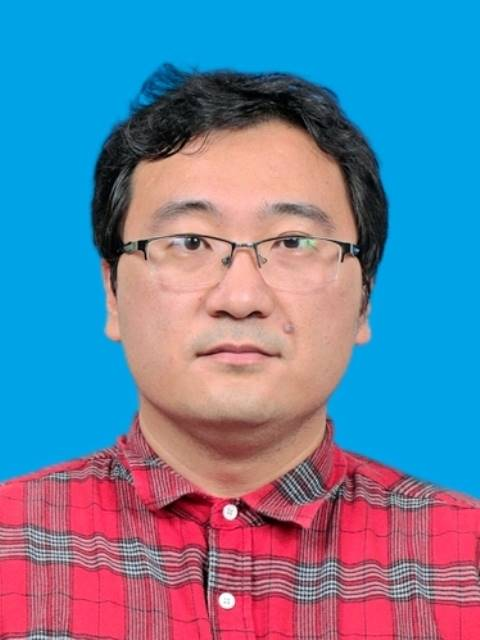
\includegraphics[width=0.65\textwidth]{./assets/thales.jpg}\hfill\null

\vspace*{0.5ex} % Extra space after the picture

\headleft{Profile}
With \textbf{20 years of development experience}, \textbf{15 years in leadership roles}, and \textbf{5 years specializing in artificial intelligence}, I bring a unique blend of technical expertise and strategic vision. I am deeply passionate about R\&D, consistently staying at the forefront of industry trends. My strong research capabilities have led to multiple successful \textbf{technology-to-industry implementations} from academic papers. I have managed teams of over 100 members, delivering complex projects with efficiency, innovation, and sustainable impact.
% 20年开发经验，15年管理经验，5年人工智能经验。对研发一直赋予极大的热爱，时刻关注行业内最新动态。拥有很强的科研能力，做过多次论文落地。管理过上百人的团队，拥有丰富的管理经验。

\headleft{Personal information}
\small % To fit more content
\emph{Ph.D. Candidate in Intelligent Science and Systems} \\[0.4ex]
\MVAt\ {\small jiangtai20@mails.ucas.ac.cn} \\[0.4ex]
\Mobilefone\ +86\,138\,1093\,5087 \\[0.5ex]
\Letter\ 1st Xi'erqi road, Haidian, Beijing
\normalsize


\headleft{Skills}
\begin{itemize}
\item Server, DevOps
\item Frontend, 3D
\item Blockchain, Web3
\item AI, ML, DL, RL
\item Team Managing
\end{itemize} 

\headleft{Hobbies}
\textit{Sport:} Badmnton, Sketing, Bowling, Archery.

\textit{Miscellaneous:} Astronomy, Zoology, Consumer Psychology.



\end{minipage}%
\kern0.09\textwidth\relax%%Right margin provided explicitly to stretch the colourbox
}
\end{minipage}% Right column
\hskip2.5em% Left margin for the white area
\begin{minipage}[t]{0.56\textwidth}
\setlength{\parskip}{0.8ex}% Adds spaces between paragraphs; use \\ to add new lines without this space. Shrink this amount to fit more data vertically

\vspace{2ex}

\headright{Works}
% 带领科研团队完成论文落地，主要涉及图像识别，语音识别，大模型应用，去中心化科学

\textsc{Architecture} at \textbf{Institute of Automation, Chinese Academy of Sciences.}  \dates{2019.7--pres.} \\
\smaller{Lead research team in projects involving image recognition, speech recognition, large language model applications, and decentralized science (DeSci).} \\
\smaller{Designed and implemented frameworks for blockchain, DAO governance, smart contracts, Web3.0, and recursive inscriptions.} \\
\smaller{Applied reinforcement learning to route planning, simulation, and engineering optimization.} \\
\smaller{Developed solutions in multi-object detection, augmented reality, and 3D reconstruction, achieving successful real-world deployments.}



\is % Item spacing -- defined in the preamble
\textsc{Architecture} at \textbf{JD.com, inc.}  \dates{2018.4--2019.7} \\
\smaller{Built and optimized enterprise software frameworks, enhancing development efficiency and cross-project consistency.}\\
\smaller{Developed auction and recycling systems from concept to production.}\\
\smaller{Created a reusable component library adopted across multiple teams.}\\
\smaller{Managed and coordinated a team of 100+ members, ensuring timely delivery of high-quality products.}

% 开发拍卖系统。开发回收系统。构件公用组件库。管理百人团队。

\is
\textsc{CTO} at \textbf{Vogso Ltd.\ (Hong Kong).}  \dates{2010.8--2018.3} \\
\smaller{Led system architecture, technology selection, and product development for web and game platforms.}\\
\smaller{Established and scaled a high-performing development team, opening a new branch office to support expansion.}\\
\smaller{Oversaw project delivery, ensuring performance optimization and long-term maintainability.}

\is
\textsc{Engineering} at \textit{Our Palm inc.} \dates{2008.3--2010.7} \\
\smaller{Developed real-time combat systems for online games, achieving 10,000+ daily active users.}\\
\smaller{Optimized database performance and gameplay systems to improve user engagement.}

\is
\textsc{Lecturer} at \textit{Xinhua Computer College.} \dates{2004.4--2008.3} \\
\smaller{Taught web development and computer fundamentals to undergraduate students.}\\
\smaller{Developed teaching materials and improved curriculum delivery.} 


\headright{Education}

\textsc{Ph.D. degree with the Institute of System Engineering.} Intelligent Science and Systems. \textit{Macau University of Science and Technology}. \dates{2023--2026} \\
% \smaller{Thesis title: \textit{Journal DAO: User-Incentivized Autonomous Decentralized Scientific Publishing in Web3.}} \\
\smaller{Conducted research integrating large-scale AI models with blockchain, delivering solutions successfully applied in industry, agriculture, and publishing.}
% 做出了多种大模型结合区块链的成果，成果在工业，农业，出版业落地

\is
\textsc{Master.} Artificial Intelligence and Application. \textit{University of Chinese Academy of Sciences}. \dates{2020--2022} \\
\smaller{Thesis title: \textit{Smart Resale Based on Multi-Object Detection and Augmented Reality.}} \\
\smaller{Achieved GPA 3.9 (top of class) in machine learning, deep learning, and reinforcement learning.}\\
\smaller{Contributed to teaching materials and designed an AlphaGo lesson plan still in active use.}
% 钻研了机器学习，深度学习，强化学习等人工智能基础知识，各科成绩名列前茅，GPA3.9，并协助编写了教材，制作了沿用至今的AlphaGo教案

\is
\textsc{Bachelor.} Computer Network. \textit{Xijing University}.  \dates{2001--2005} \\
\smaller{Won First Prize in the city-level C Language Competition.} \\
\smaller{Earned CCNA Network Engineer certification.}
% 学习了各种计算机相关知识，C语言参加市级大赛获一等奖，考取了ccna网络工程师



\end{minipage}

\end{document}